\chapter{Google Analytics}
\label{chap:ga}

% Describe Google Accounts, Google Analytics Accounts, Web properties, profiles/views, etc. 

% Google Analytics hierarchy is illustrated in Figure~\ref{fig:Hierarchy} \cite{Hiera14:online}.
\begin{figure}[h]
  \centering
  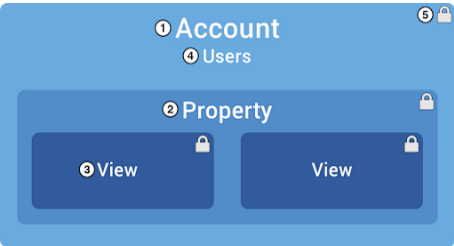
\includegraphics[width=.5\textwidth]{figures/Hierarchy.png}
  \caption[Hierarchy]{Hierarchy of accounts, users, properties, and views.}
  \label{fig:Hierarchy}
\end{figure}
\section{Google Account}
The Google account is the user account that provides access to several Google services. To use these services it is required to create a Google account. As seen in Figure~\ref{fig:Hierarchy}, this account is the access point for Google Analytics and the top-most level of this service \cite{Hiera14:online}. To use Google Analytics, it is required to use at least one account, which will allow to identify the properties to be tracked. The relationship between accounts and properties may vary depending on the user. 


This Google account can also be used to access other Google services such a Gmail, Youtube, etc.
\section{Web Property}
\label{sec:webProperty}
A web property (also referred to as property) is a website, mobile application or device. There are different types of websites, which include social media accounts, blogs, news websites, etc. One account can contain one or more web properties. To add a web property and collect data, it has to be added within an analytics account.
Google Analytics sees a property only as a resource associated with a tracking code \cite{About27:online}. A tracking code contains a unique ID that identifies which web property the tracking data belongs to. When a resource is being tracked using Google Analytics (For example a website), there is a property ID included in the tracking code in the website source code or inside the app \cite{About27:online}. 
Analytics will then create unfiltered views for each property that is added. There is a limit of 25 properties which can be added to one Analytics account.

\section{Views}
A view (also referred to as profile) is the access point for reports; a defined view of data from a property \cite{Hiera14:online}. In other words, views allows organization and filtering of report data. Google will automatically create one unfiltered view for every web property added in the account. But this can be changed by adding multiple views in a single web property. The first view which is created is without filters and includes all the data of that selected property. Creating additional views and using the filters to customize the reports and see only a subset of data and not the whole unfiltered data collected. Web and apps views are two different types of views which give a slightly different analysis experience. App views can show some reports which are not available in web views and vice-versa  \cite{About20:online}. However, the usage of them is based on what kind of data is collected and the system being used.
As in the web properties, there is also a limit of 50 views for each property.